
El motor seleccionado es el~\cite{EMG30datasheet}.
Se dispone de conocimiento previo de su uso y características facilitando el trabajo.
En aspecto del motor se aprecia en la~\cref{fig:EMG Motor}.
Cumple con los requerimientos de ser sencillo, barato y disponer de una calidad suficiente para ejercer el control PID.

Los parámetros que definen sus características más relevantes se encuentran en la~\cref{tab:EMG30specifications}.
El código de colores de las conexiones se extraen en la~\cref{fig:motor connection}

\begin{figure}[H]
    \centering
    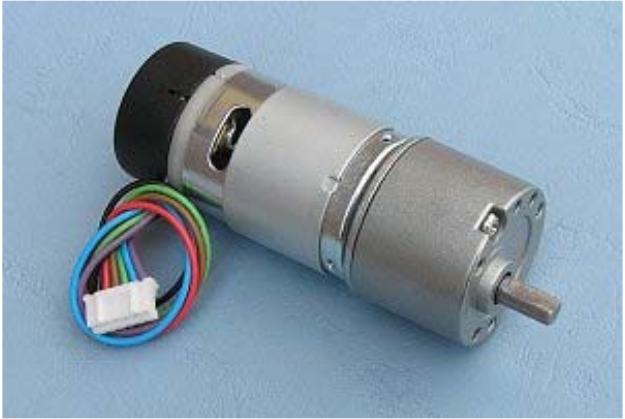
\includegraphics[scale = 0.35]{part/Proyecto_ejecutivo/memoria_constructiva/motor/img/MotorEMG30}
    \caption{Motor EMG30\cite{EMG30datasheet}}\label{fig:EMG Motor}
\end{figure}

\begin{figure}[H]
    \centering
    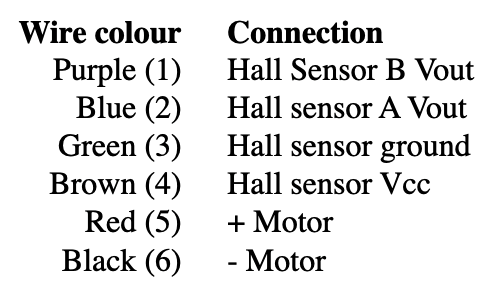
\includegraphics[scale = 0.5]{part/Proyecto_ejecutivo/memoria_constructiva/motor/img/motorConnection}
    \caption{Motor EMG30 \\Fuente: Documento de especificaciones técnicas.\cite{EMG30datasheet}}\label{fig:motor connection}
\end{figure}

\begin{table}[H]
    \centering
    \caption{Características EMG30 Fuente:\cite{EMG30datasheet}}\label{tab:EMG30specifications}
    \begin{tabular}{|l|l|}
        \hline
        Característica & Valor\\
        \hline
        Voltaje nominal & 12 V\\
        \hline
        Torque nominal & 1.5 kg/cm\\
        \hline
        Velocidad nominal & 170 rpm\\
        \hline
        Intensidad nominal & 530 mA\\
        \hline
        Velocidad sin carga& 216 rpm\\
        \hline
        Intensidad sin carga& 150mA\\
        \hline
        Intensidad máxima& 2.5 A\\
        \hline
        Salida nominal & 4.22 W\\
        \hline
        Pasos por vuelta del codificador& 360 \\
        \hline
        Razón de la reductora & 30:1\\
        \hline
    \end{tabular}
\end{table}



